\documentclass[11pt]{article}
\usepackage[margin=1in]{geometry}
\usepackage{booktabs}
\usepackage{graphicx}
\usepackage{natbib}
\usepackage[hidelinks]{hyperref}

\title{Site-specific PM2.5 changes in a synthetic before--after monitoring exercise}
\author{Anonymous teaching example}
\date{}

\begin{document}
\maketitle

\begin{abstract}
Pooled summaries can hide differences between monitoring sites. We described 480 synthetic sensor-week observations from three sites, two study arms, and periods before and after a simulated intervention. Mean PM2.5 in the intervention arm changed from 37.02 to 34.36~$\mu$g/m$^3$, while the comparison arm changed from 37.64 to 38.32~$\mu$g/m$^3$. North and Central intervention means decreased, whereas the South intervention mean increased from 29.22 to 34.56~$\mu$g/m$^3$. The exercise supports site-stratified descriptive reporting but does not support causal claims.
\end{abstract}

\section{Introduction}
Overall before--after averages may conceal site heterogeneity \citep{Arun2024CommunityPM}. Repeated sensor observations also require attention to temporal structure and dependence \citep{Chen2023SensorWeeks}. This teaching report demonstrates claim calibration with a synthetic dataset.

\section{Data and Methods}
The dataset contained 480 observations from North, Central, and South sites. Each site included intervention and comparison arms, eight weeks before and eight weeks after a simulated intervention, and five sensor identifiers per arm-week. We calculated descriptive means by site, arm, and period. The exercise did not provide a random assignment mechanism, calibration records, covariates, or an inferential model.

\section{Results}
The intervention-arm mean changed from 37.02 to 34.36~$\mu$g/m$^3$; the comparison-arm mean changed from 37.64 to 38.32~$\mu$g/m$^3$. Intervention means decreased in North (44.42 to 35.50) and Central (37.41 to 33.01), while the South mean increased (29.22 to 34.56).

\begin{figure}[htbp]
  \centering
  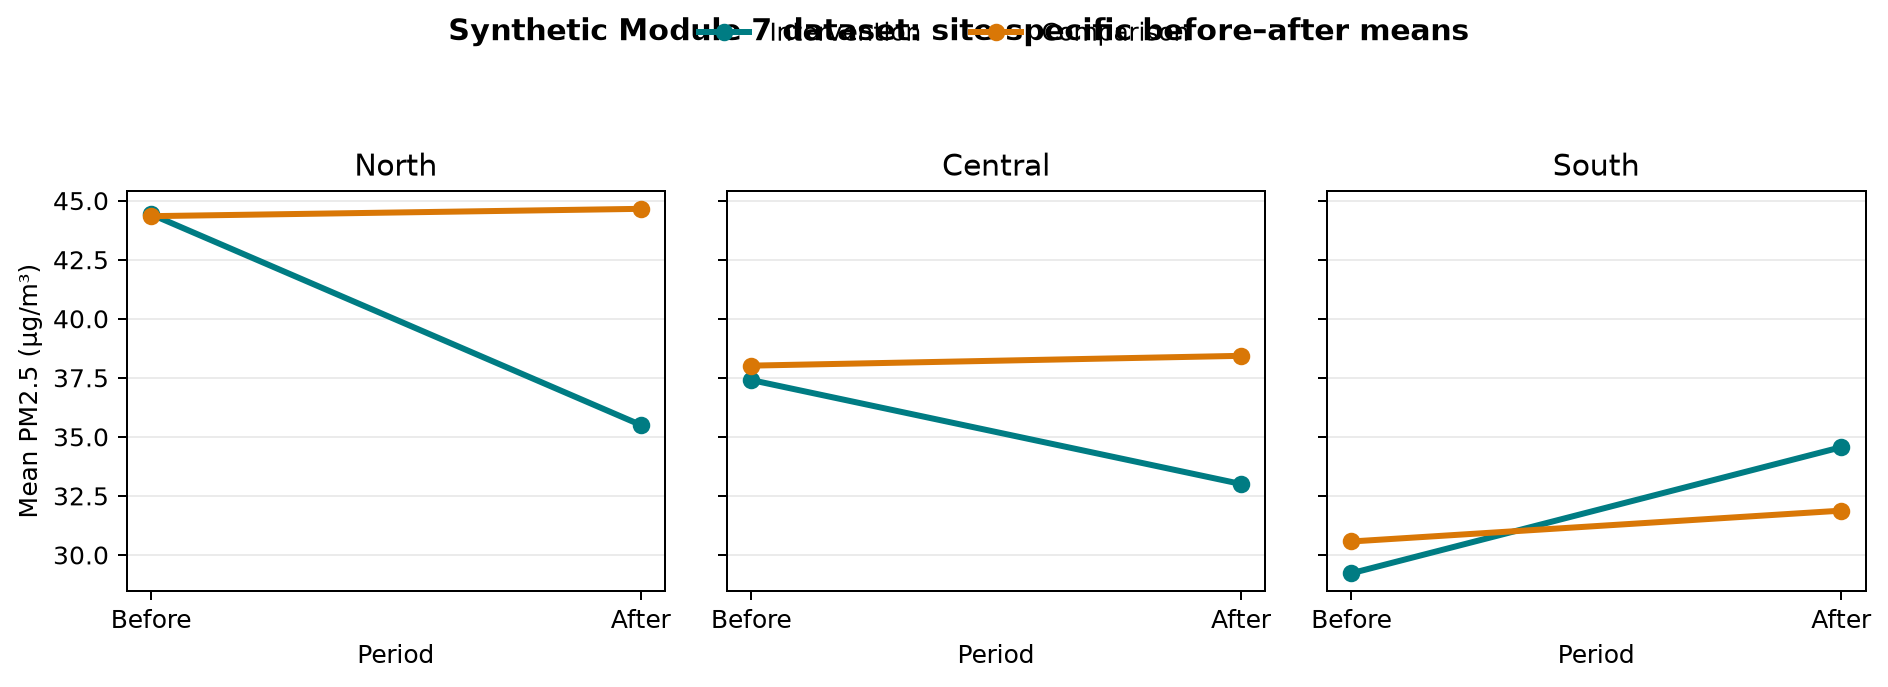
\includegraphics[width=\linewidth]{course-materials/document-production/figures/pm25-before-after.png}
  \caption{Site-specific before--after means from the synthetic Module 7 dataset. Lines are descriptive summaries and do not show causal effects or uncertainty.}
\end{figure}

\section{Discussion}
The pooled decrease in the intervention arm does not represent every site. South changed in the opposite direction, so a report limited to the overall mean would overstate consistency. Causal language would exceed the available design evidence \citep{Diaz2025BeforeAfter}.

\section{Limitations}
The data are synthetic. The exercise lacks assignment details, calibration records, covariates, missing-data context, and uncertainty estimates that account for repeated sensor-week observations.

\section{Conclusion}
The dataset supports a descriptive conclusion that PM2.5 patterns differed by site. Additional design and measurement evidence would be required to attribute changes to the simulated intervention.

\bibliographystyle{plainnat}
\bibliography{module-08-mock-references}
\end{document}
